\section{Sequence-to-Sequence with RNNs}
\begin{frame}{}
    \LARGE Advanced Computer Vision: \textbf{Sequence-to-Sequence with RNNs}
\end{frame}

\begin{frame}[allowframebreaks]{Sequence-to-Sequence with RNNs}
    \begin{figure}
    \centering
    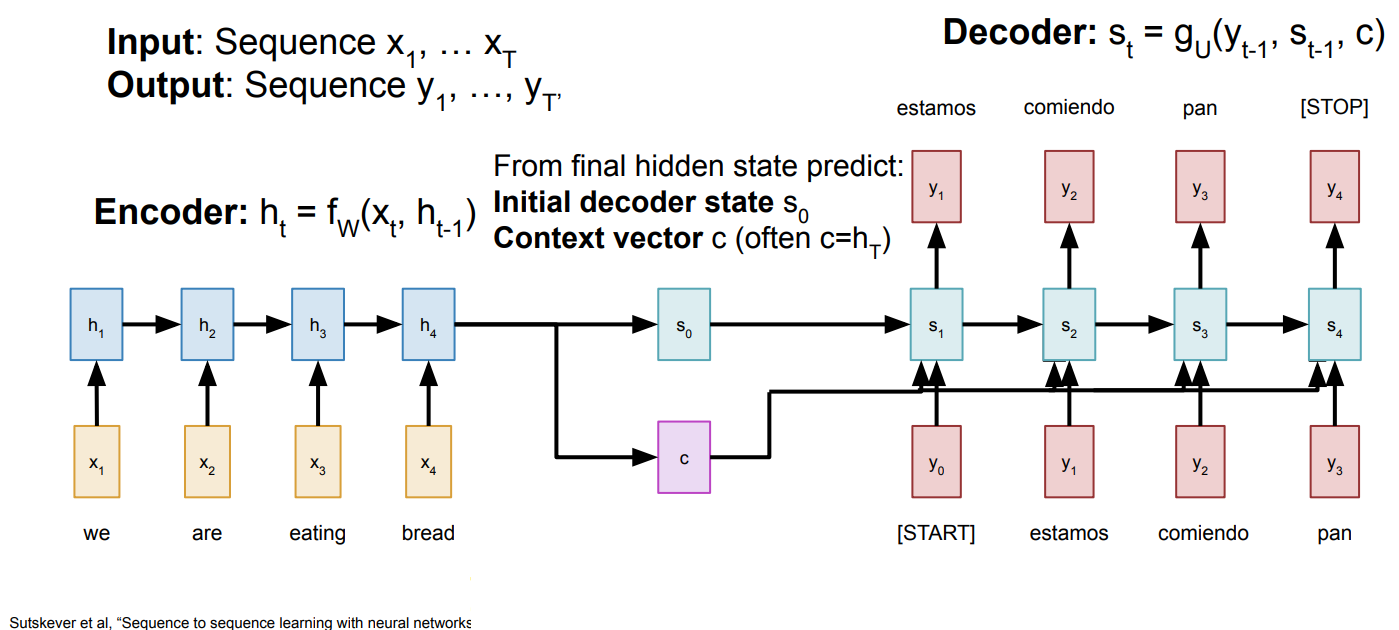
\includegraphics[width=1.0\textwidth,height=1.0\textheight,keepaspectratio]{images/advanced-cv/rnn_5.png}
    \end{figure}  
\framebreak
    \begin{figure}
    \centering
    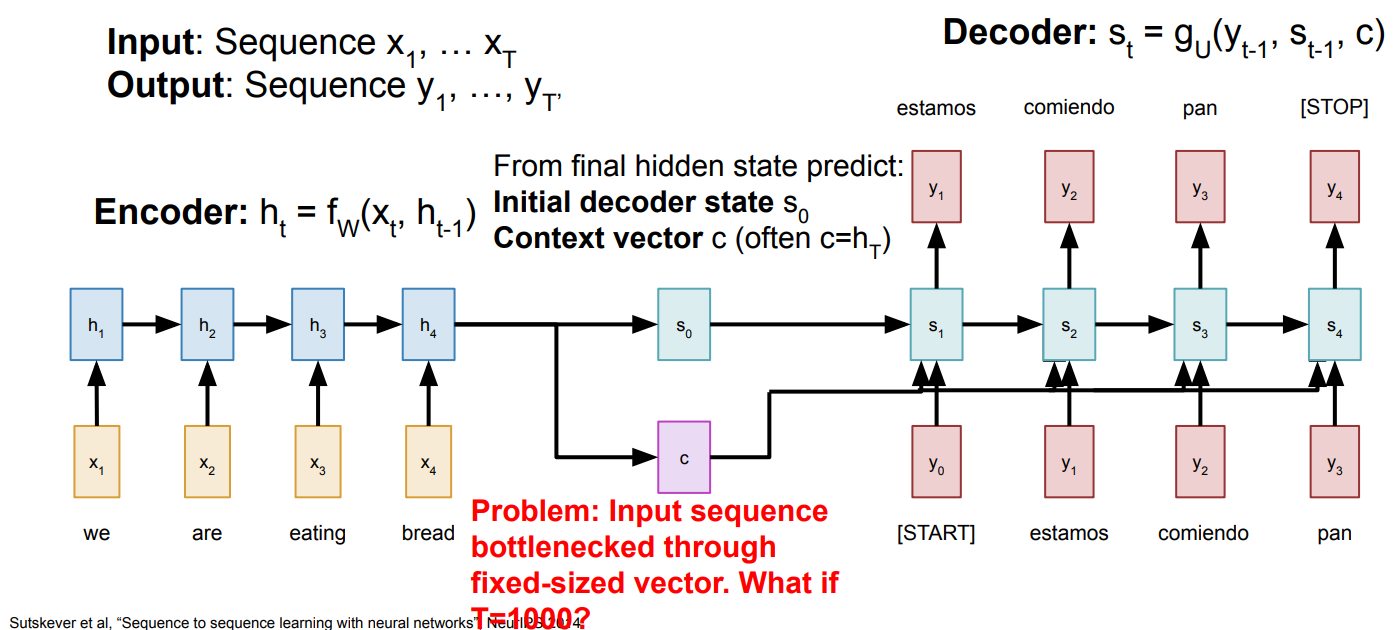
\includegraphics[width=1.0\textwidth,height=1.0\textheight,keepaspectratio]{images/advanced-cv/rnn_6.png}
    \end{figure}  
\framebreak
    \begin{figure}
    \centering
    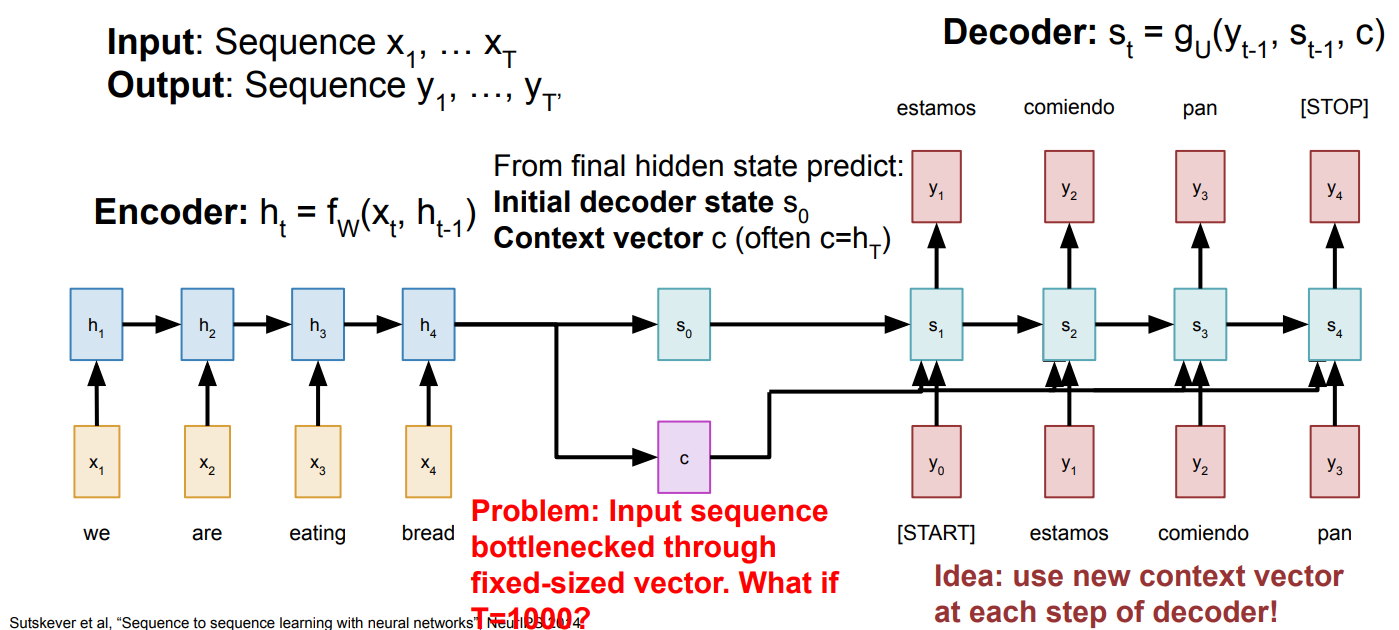
\includegraphics[width=1.0\textwidth,height=1.0\textheight,keepaspectratio]{images/advanced-cv/rnn_7.png}
    \end{figure}     
\end{frame}

\begin{frame}{Introduction to Attention}
    \begin{itemize}
        \item \textbf{Key idea:} “Don’t process everything — just focus on the most relevant parts.”
        \item Attention helps models decide where to look in a sequence.
    \end{itemize}
    \vspace{1em}
    \textbf{Equation (simplified):}
    \begin{align*}
        \text{Attention}(Q, K, V) = \mathrm{softmax}\left(\frac{QK^\top}{\sqrt{d_k}}\right)V
    \end{align*}
    \begin{itemize}
        \item $Q$ = Queries
        \item $K$ = Keys
        \item $V$ = Values
    \end{itemize}
\end{frame}

\begin{frame}[allowframebreaks]{Sequence-to-Sequence with RNNs and Attention}
    \begin{figure}
    \centering
    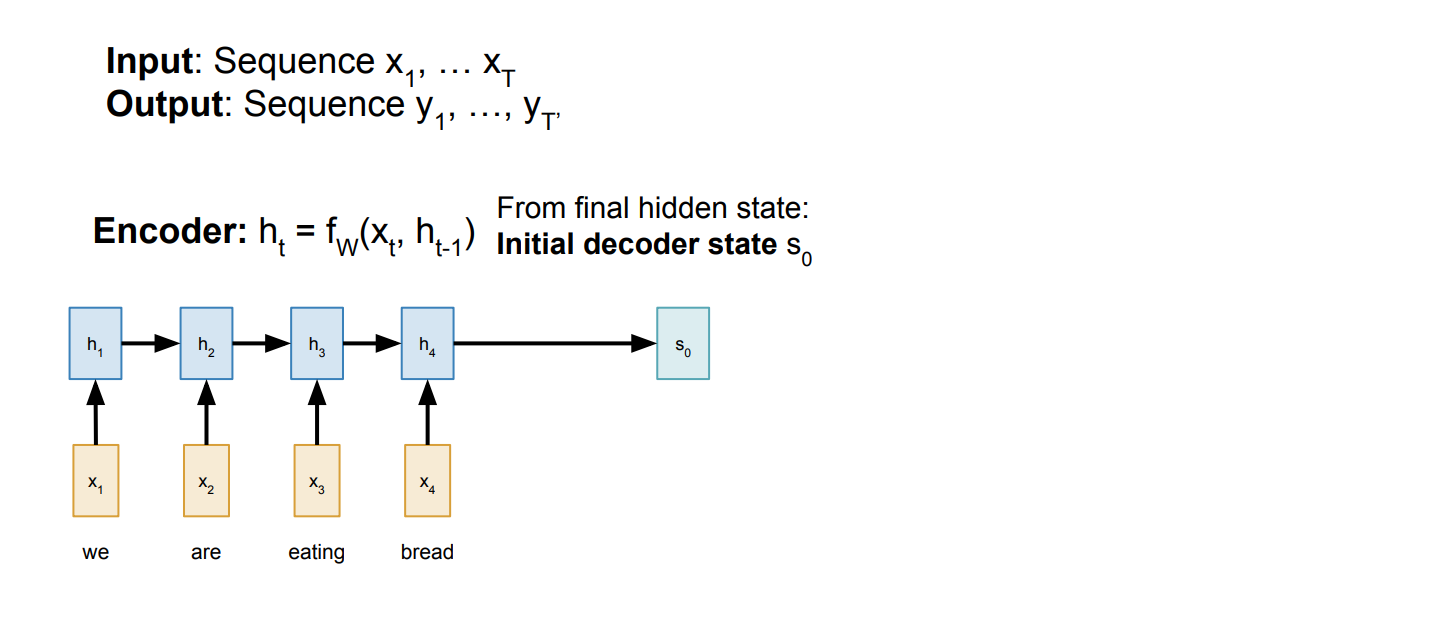
\includegraphics[width=1.0\textwidth,height=1.0\textheight,keepaspectratio]{images/advanced-cv/attention_1.png}
    \end{figure}  
\framebreak
    \begin{figure}
    \centering
    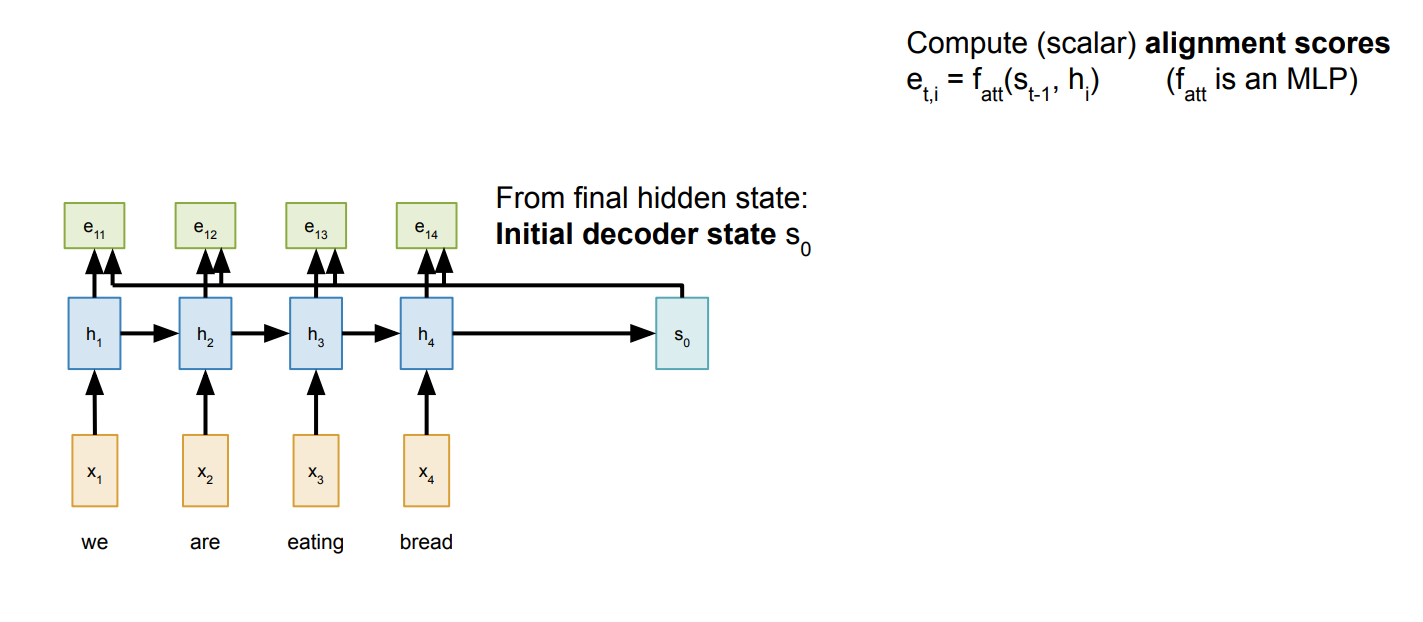
\includegraphics[width=1.0\textwidth,height=1.0\textheight,keepaspectratio]{images/advanced-cv/attention_2.png}
    \end{figure}  
\framebreak
    \begin{figure}
    \centering
    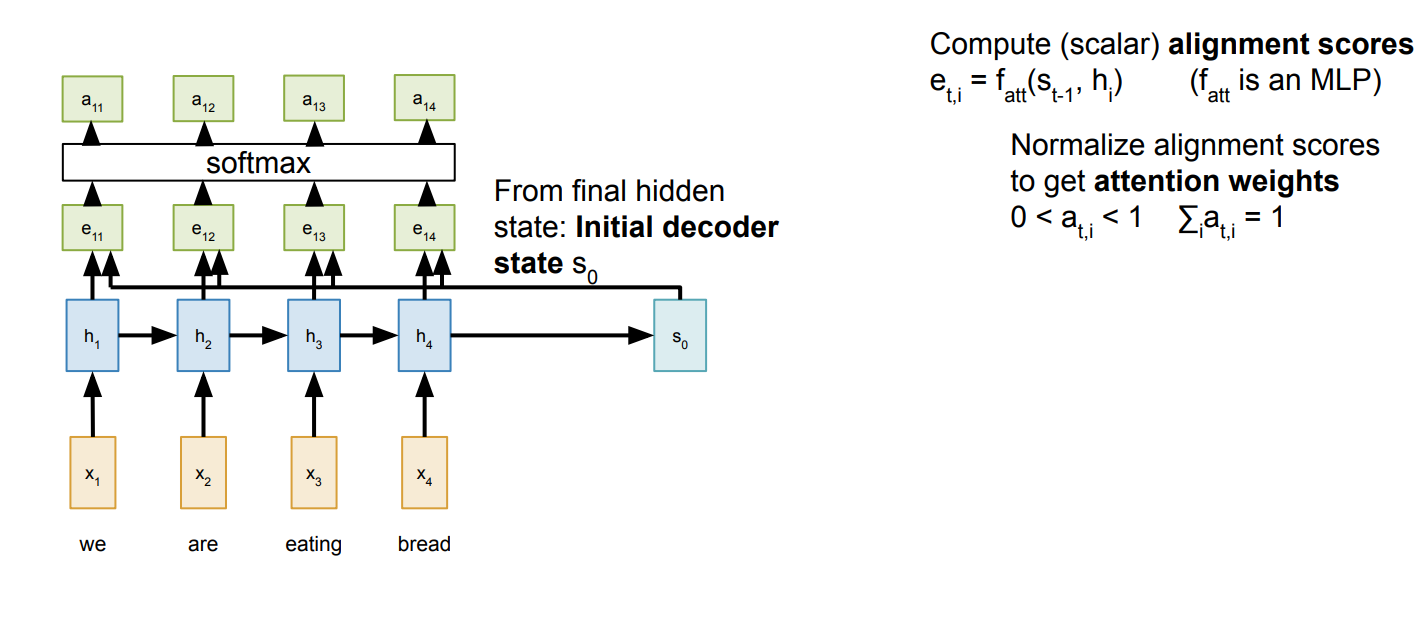
\includegraphics[width=1.0\textwidth,height=1.0\textheight,keepaspectratio]{images/advanced-cv/attention_3.png}
    \end{figure}  
\framebreak
    \begin{figure}
    \centering
    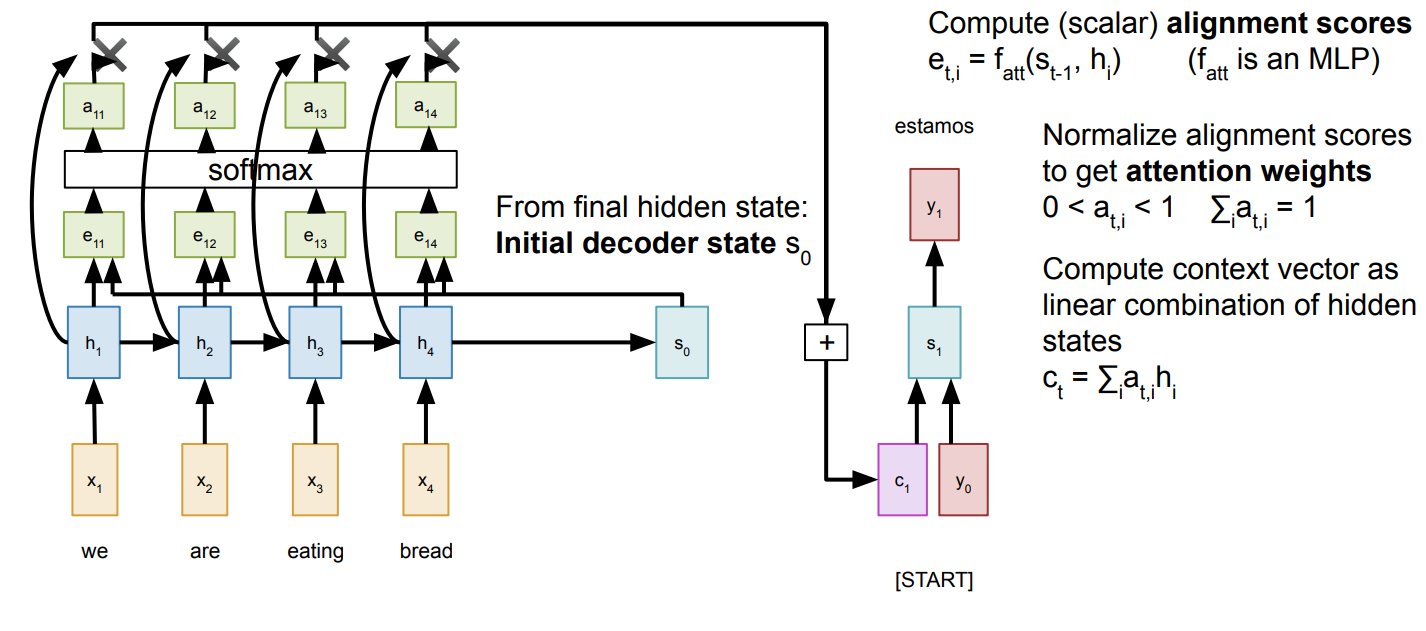
\includegraphics[width=1.0\textwidth,height=1.0\textheight,keepaspectratio]{images/advanced-cv/attention_4.png}
    \end{figure}  
\framebreak
    \begin{figure}
    \centering
    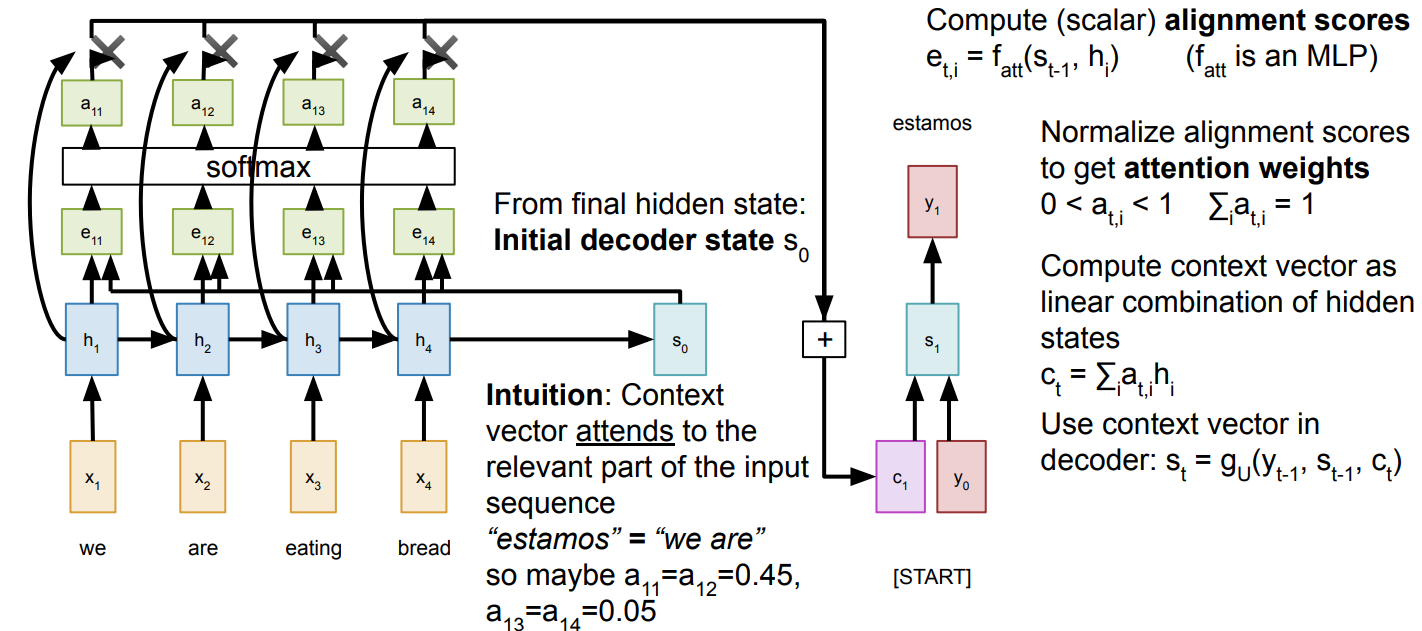
\includegraphics[width=1.0\textwidth,height=1.0\textheight,keepaspectratio]{images/advanced-cv/attention_5.png}
    \end{figure}  
\framebreak
    \begin{figure}
    \centering
    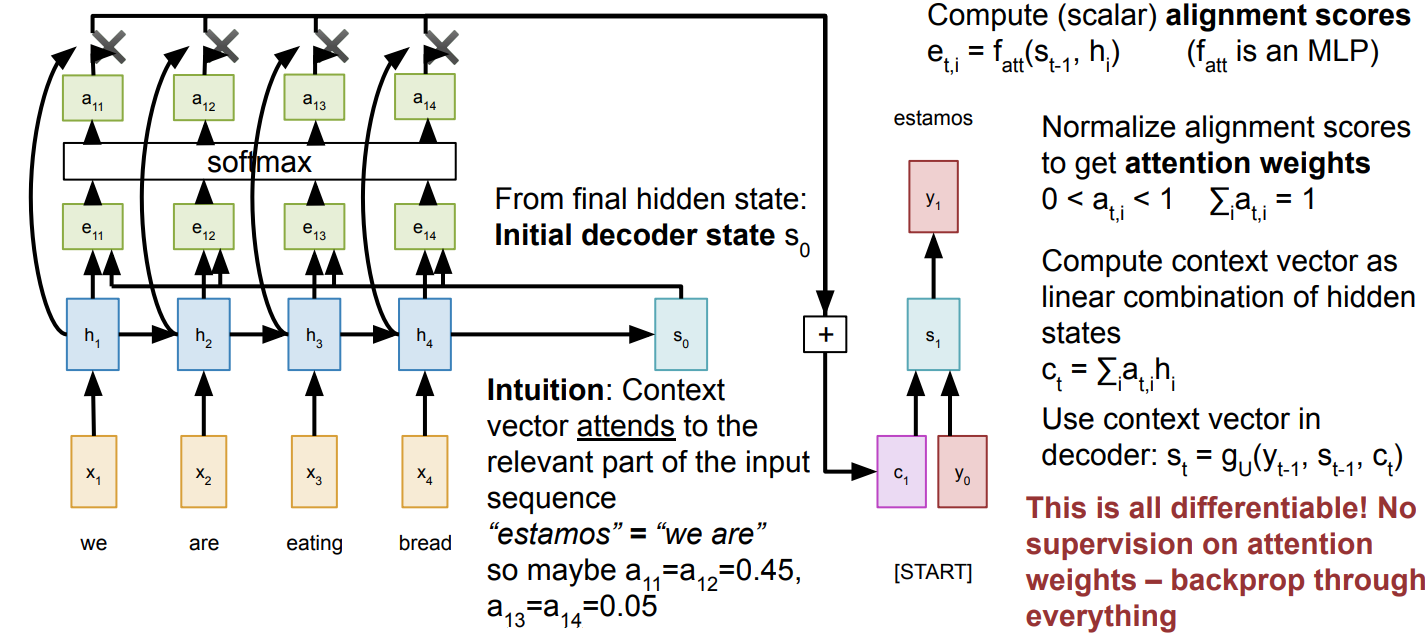
\includegraphics[width=1.0\textwidth,height=1.0\textheight,keepaspectratio]{images/advanced-cv/attention_6.png}
    \end{figure}  
\framebreak
    \begin{figure}
    \centering
    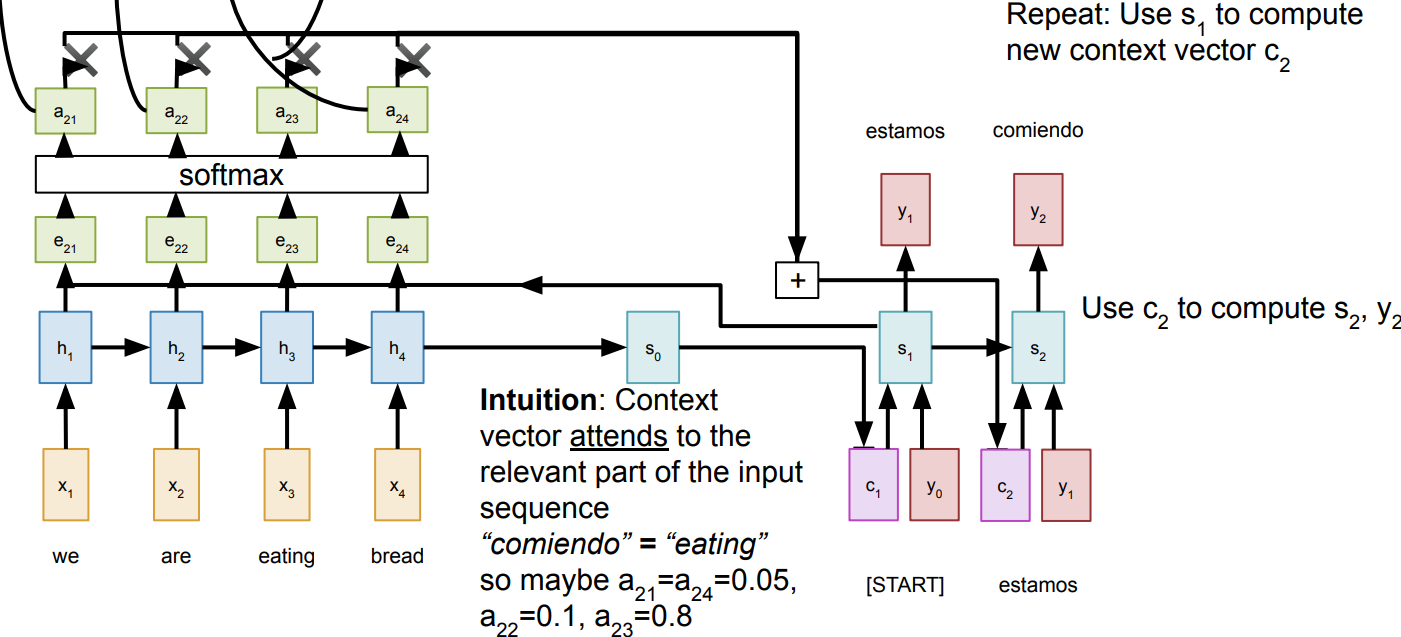
\includegraphics[width=1.0\textwidth,height=1.0\textheight,keepaspectratio]{images/advanced-cv/attention_7.png}
    \end{figure}  
\framebreak
    \begin{itemize}
        \item Use a different context vector at each timestep of the decoder.
        \item The input sequence is not bottlenecked through a single vector.
        \item At each timestep of the decoder, the context vector "looks at" different parts of the input sequence.
    \end{itemize}
    \begin{figure}
    \centering
    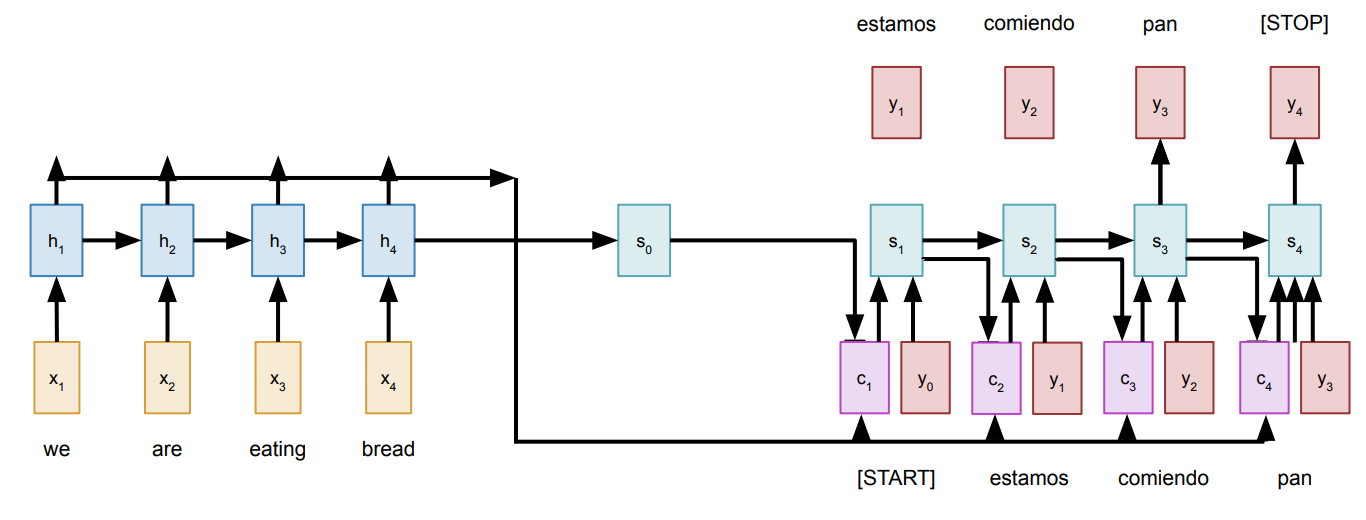
\includegraphics[width=1.0\textwidth,height=0.6\textheight,keepaspectratio]{images/advanced-cv/attention_8.png}
    \end{figure}  
\framebreak
    \begin{figure}
    \centering
    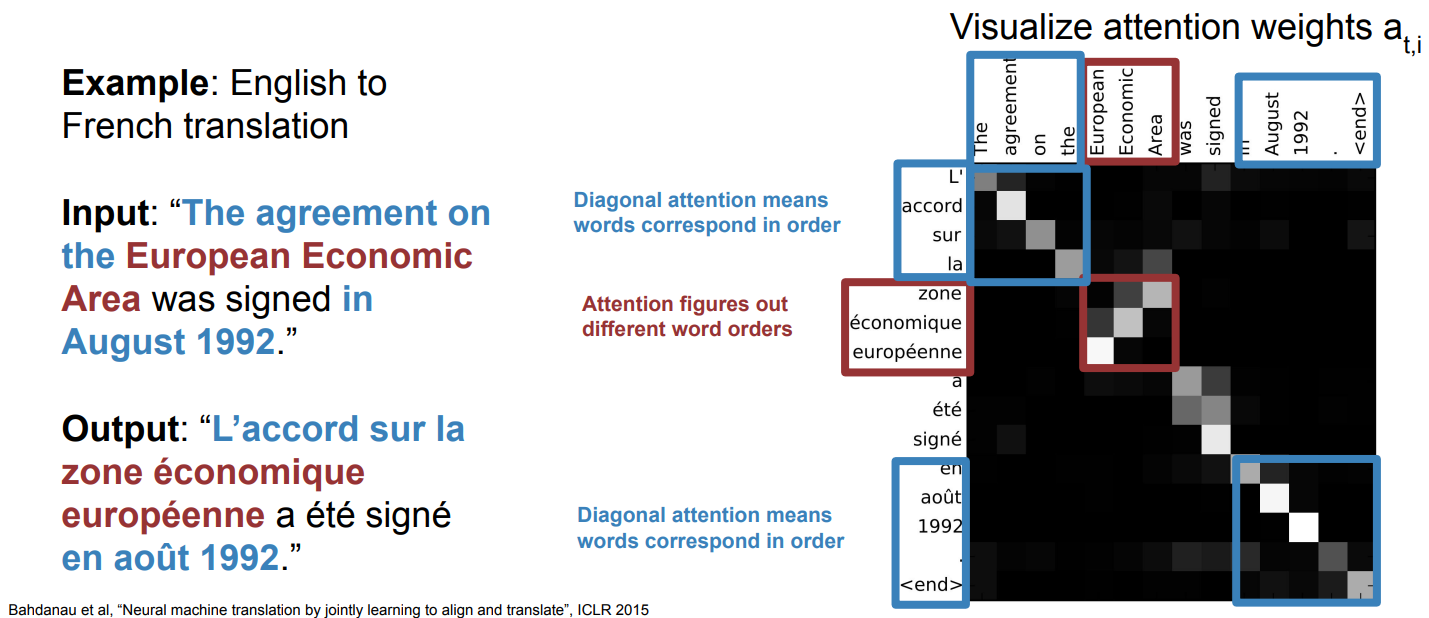
\includegraphics[width=1.05\textwidth,height=1.0\textheight,keepaspectratio]{images/advanced-cv/attention_9.png}
    \end{figure} 
\end{frame}